\documentclass[a4paper,11pt,oneside]{report}

\usepackage[UKenglish]{babel}

\usepackage{xcolor}
\usepackage{graphicx}

\usepackage{caption}

\begin{document}
\makebox[1\textwidth][c]{
\begin{tabular}{ccccccc}

\includegraphics{../SPM/examples/slots/squared_slot} &
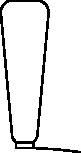
\includegraphics{../SPM/examples/slots/rounded_slot} &
\includegraphics{../SPM/examples/slots/round_slot} &
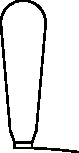
\includegraphics{../SPM/examples/slots/semiround_slot} &
\includegraphics{../SPM/examples/slots/roundsemi_slot} &

\includegraphics{../SPM/examples/slots/semiarc_slot} &

\includegraphics{../SPM/examples/slots/roundarc_slot} \\
%
\texttt{squared} &
\texttt{rounded} &
\texttt{round} &
\texttt{semiround} &
\texttt{roundsemi} &
\texttt{semiarc} & 
\texttt{roundarc}
\end{tabular}}
\vspace{1cm}

\begin{tabular}{c}
\includegraphics[scale=0.5]{../SPM/examples/stators/1pole} 
\\
$ 1 $ \texttt{pole}
\end{tabular}
\vspace{5mm}

\begin{tabular}{c}
\includegraphics[scale=0.5]{../SPM/examples/stators/2pole} 
\\
$ 2 $ \texttt{poles}
\end{tabular}
\vspace{5mm}

\begin{tabular}{c}
\includegraphics[scale=0.5]{../SPM/examples/stators/ppole} 
\\
$ p $ \texttt{poles}
\end{tabular}
\vspace{5mm}

\begin{tabular}{c}
\includegraphics[scale=0.5]{../SPM/examples/stators/2ppole} 
\\
$ 2p $ \texttt{poles}
\end{tabular}

\end{document}